\documentclass[11pt,a4paper]{article}

\usepackage[T1]{fontenc}
\usepackage[utf8]{inputenc}
\usepackage{lmodern}
\usepackage[english]{babel}
\usepackage[a4paper,margin=2.6cm]{geometry}
\usepackage{setspace}
\usepackage{microtype}
\usepackage{parskip}
\usepackage{graphicx}
\usepackage{tikz}
\usetikzlibrary{positioning,arrows.meta,shapes.geometric}
\usepackage{booktabs}
\usepackage{longtable}
\usepackage{array}
\usepackage{tabularx}
\usepackage{enumitem}
\usepackage{xcolor}
\usepackage{hyperref}
\usepackage[nameinlink,noabbrev]{cleveref}
\usepackage{fancyhdr}
\usepackage{titlesec}
\usepackage{listings}
\usepackage{caption}

\onehalfspacing
\setlength{\headheight}{14pt}
\pagestyle{fancy}
\fancyhf{}
\fancyhead[L]{HeptaFlow Whitepaper}
\fancyhead[R]{\thepage}
\renewcommand{\headrulewidth}{0.4pt}

\definecolor{hfblue}{RGB}{25,76,132}
\definecolor{codebg}{RGB}{248,248,248}

\hypersetup{
  colorlinks=true,
  linkcolor=hfblue,
  urlcolor=hfblue,
  citecolor=hfblue,
  pdftitle={From Legacy ETL to Data Products},
  pdfauthor={Pavel Saratchev},
  pdfsubject={Generator-Based Data Platform Modernization},
  pdfkeywords={HeptaFlow, Databricks, ETL, Data Products, Migration, Spark}
}

\titleformat{\section}
  {\normalfont\Large\bfseries\color{hfblue}}
  {\thesection}{0.75em}{}

\titleformat{\subsection}
  {\normalfont\large\bfseries}
  {\thesubsection}{0.75em}{}

\titleformat{\subsubsection}
  {\normalfont\normalsize\bfseries}
  {\thesubsubsection}{0.75em}{}

\setlist[itemize]{topsep=4pt,itemsep=3pt}
\setlist[enumerate]{topsep=4pt,itemsep=3pt}

\lstdefinestyle{hfcode}{
  basicstyle=\ttfamily\small,
  backgroundcolor=\color{codebg},
  frame=single,
  framerule=0.3pt,
  rulecolor=\color{black!20},
  breaklines=true,
  columns=fullflexible,
  keepspaces=true,
  showstringspaces=false
}

\tikzset{
  hfbox/.style={
    rectangle,
    draw=black!55,
    rounded corners=2pt,
    thick,
    minimum width=12.6cm,
    minimum height=1.45cm,
    align=center,
    fill=hfblue!4
  },
  hfsmall/.style={
    font=\small
  },
  hfarrow/.style={
    -{Stealth[length=3mm,width=2mm]},
    thick,
    draw=black!70
  }
}

\newcommand{\papertitle}{From Legacy ETL to Data Products}
\newcommand{\papersubtitle}{A Generator-Based Approach to Scalable Data Platform Modernization}
\newcommand{\paperauthor}{Pavel Saratchev}
\newcommand{\paperaffiliation}{HeptaFlow / Independent Whitepaper Draft}
\newcommand{\paperdate}{\today}

\begin{document}

\begin{titlepage}
  \centering
  \vspace*{2.5cm}

  {\Huge\bfseries \papertitle \par}
  \vspace{0.6cm}
  {\Large \papersubtitle \par}

  \vspace{2.0cm}

  {\large \paperauthor \par}
  \vspace{0.2cm}
  {\normalsize \paperaffiliation \par}
  \vspace{0.2cm}
  {\normalsize \paperdate \par}

  \vfill

  \begin{minipage}{0.88\textwidth}
  \small
  \textbf{Abstract.}
  Many organizations are currently transitioning from traditional on-premise data warehouse environments toward modern cloud-based data platforms such as Databricks. In practice, this shift is often treated primarily as a technical migration, where existing ETL processes are reimplemented in a new technology stack without fundamentally addressing the structural limitations of legacy systems. The result is a familiar pattern: modern infrastructure, but legacy complexity.

  This paper presents a generator-based approach to data platform modernization in which existing ETL logic is not manually rewritten, but systematically transformed into modern data pipelines using metadata and deterministic transformation rules. The approach combines the pragmatic benefits of lift-and-shift with the structural control required for scalable modernization. It preserves validated business logic, improves consistency and repeatability, and establishes a foundation for more transparent, maintainable, and data product-oriented architectures.
  \end{minipage}

  \vfill

  \begin{minipage}{0.88\textwidth}
  \footnotesize
  \textbf{Note.}
  This paper describes architectural concepts and transformation patterns derived from real-world enterprise modernization work. Specific customer names, internal process identifiers, and implementation details have been intentionally abstracted.
  \end{minipage}
\end{titlepage}

\tableofcontents
\newpage

\section{Executive Summary}

Many organizations are currently undergoing a transition from traditional on-premise data warehouse environments—often built on Oracle, Informatica, DataStage, or similar technologies—towards modern, cloud-based data platforms such as Databricks.

While this shift is widely recognized as necessary, the approach taken is often limited to a technical migration: existing ETL processes are reimplemented in a new technology stack without fundamentally addressing the structural limitations of legacy systems.

This results in a familiar outcome: \emph{modern infrastructure, but legacy complexity}.

This paper argues that the primary challenge in such transformations is not the technology itself, but the way data processing logic is defined, structured, and maintained.

We present a generator-based approach to data platform modernization in which existing ETL logic is not manually rewritten, but systematically transformed into modern data pipelines using metadata and deterministic transformation rules.

This approach enables:
\begin{itemize}
  \item consistent and repeatable transformation of legacy processes,
  \item clear separation between business logic and technical execution,
  \item scalable generation of data pipelines aligned with modern data platform principles.
\end{itemize}

Rather than focusing on isolated pipeline migration, this method introduces a structured path towards data product-oriented architectures, where logic is transparent, reproducible, and maintainable across systems.

\section{Introduction}

In many enterprise environments, data platforms have evolved over years or decades into highly complex ecosystems. Business-critical logic is embedded in ETL tools, database procedures, and custom scripts, often without clear documentation or ownership.

These systems are stable, but difficult to change.

With the adoption of cloud-based platforms such as Databricks, organizations aim to modernize their data landscape. However, the migration challenge is not only technical. It is fundamentally structural.

Rebuilding legacy ETL processes manually in a new environment is time-consuming, error-prone, and often leads to a replication of existing problems in a different technology stack.

A more systematic approach is required.

\section{The Problem: Legacy ETL at Scale}

In many organizations, data warehouse environments have grown incrementally over long periods of time. What initially started as a structured system to support reporting and analytics has evolved into a complex network of tightly coupled data pipelines, transformations, and dependencies.

These systems are not inherently flawed. On the contrary, they often represent years of accumulated domain knowledge and have proven to be stable and reliable in production.

However, their structure presents significant challenges when it comes to change and modernization.

\subsection{Fragmented and Tool-Centric Logic}

In traditional environments, business logic is distributed across multiple layers:
\begin{itemize}
  \item ETL tools (e.g.\ Informatica workflows and mappings),
  \item database procedures and SQL scripts,
  \item scheduling systems and job orchestration tools,
  \item configuration files and parameter tables.
\end{itemize}

As a result, there is no single, coherent representation of how data is transformed.

Understanding a single data flow often requires navigating multiple tools and technologies, each with its own abstraction and conventions. This fragmentation makes it difficult to analyze, validate, or systematically modify existing processes.

\subsection{Hidden Business Semantics}

A large portion of business logic is embedded implicitly within technical implementations.

Examples include:
\begin{itemize}
  \item conditional transformations encoded in ETL mappings,
  \item surrogate key generation strategies,
  \item temporal validity handling (e.g.\ slowly changing dimensions),
  \item implicit filtering logic or data quality rules.
\end{itemize}

These semantics are rarely documented in a structured way. Instead, they are hidden within code, tool configurations, or developer knowledge.

This creates a strong dependency on individuals and makes knowledge transfer difficult. It also increases the risk of introducing inconsistencies during changes or migrations.

\subsection{Tight Coupling and Low Reusability}

Legacy ETL processes are typically designed as end-to-end pipelines, where each step is tightly coupled to upstream and downstream components.

Common characteristics include:
\begin{itemize}
  \item hard-coded dependencies between jobs,
  \item direct references to physical tables and schemas,
  \item environment-specific logic embedded in code,
  \item duplication of similar transformation logic across pipelines.
\end{itemize}

This structure limits reusability and makes it difficult to isolate or evolve individual components. Even small changes can have unintended side effects across the system.

\subsection{High Cost of Change}

Due to the factors described above, modifying or migrating existing ETL processes is expensive:
\begin{itemize}
  \item changes require deep understanding of multiple tools,
  \item testing is complex and often manual,
  \item regression risks are high,
  \item documentation is incomplete or outdated.
\end{itemize}

As a result, organizations tend to avoid structural improvements and instead apply incremental fixes. Over time, this leads to increasing complexity and technical debt.

\subsection{Migration Without Transformation}

When organizations move to modern platforms, these structural issues are often carried forward.

Instead of rethinking how data processing logic is defined, existing pipelines are reimplemented using new technologies such as Spark or cloud-native services.

While this approach may reduce infrastructure constraints, it does not address the underlying problems:
\begin{itemize}
  \item logic remains fragmented,
  \item dependencies remain implicit,
  \item reusability remains limited.
\end{itemize}

In effect, legacy complexity is reproduced in a modern environment.

\subsection{Summary}

The core challenge of data platform modernization is not the migration of code, but the transformation of structure.

Without a systematic way to externalize, standardize, and control transformation logic, organizations risk rebuilding the same problems in a different technological context.

A different approach is required—one that treats transformation logic as a first-class, structured artifact rather than an implementation detail.

\section{Why Naive Lift-and-Shift Falls Short}

In many modernization initiatives, organizations adopt a lift-and-shift strategy to accelerate migration to new platforms. Existing ETL processes are translated or reimplemented in a new technology stack, with the goal of preserving existing functionality while reducing time-to-migration.

This approach is pragmatic and, in many cases, necessary.

However, when applied without structure, lift-and-shift tends to reproduce the limitations of legacy systems in a modern environment.

\subsection{Reproducing Complexity}

Without a clear abstraction of transformation logic, migration efforts focus on translating technical implementations rather than understanding underlying semantics.

As a result:
\begin{itemize}
  \item fragmented logic is carried over into new codebases,
  \item implicit dependencies remain unresolved,
  \item duplicated logic persists across pipelines.
\end{itemize}

The outcome is a system that is technically modern, but structurally unchanged.

\subsection{Loss of Control and Consistency}

Manual translation of ETL processes introduces variability:
\begin{itemize}
  \item different developers interpret logic differently,
  \item naming conventions and structures diverge,
  \item inconsistencies accumulate over time.
\end{itemize}

This makes it difficult to maintain a coherent and predictable data platform.

\subsection{High Effort, Limited Reusability}

Even when migration is successful, the resulting pipelines often remain tightly coupled and difficult to reuse.

Each pipeline is treated as an individual implementation, rather than as part of a systematic transformation framework.

This limits scalability and increases long-term maintenance effort.

\subsection{The Missing Layer: Structured Transformation}

The core issue is not the decision to migrate existing logic, but the lack of a structured mechanism to do so.

What is missing is a layer that:
\begin{itemize}
  \item explicitly represents transformation logic,
  \item separates logic from execution,
  \item ensures consistent application of patterns,
  \item enables repeatable and scalable generation of pipelines.
\end{itemize}

Without such a layer, lift-and-shift remains a manual, error-prone process.

\subsection{Summary}

Lift-and-shift is not inherently flawed.

However, without structure and abstraction, it becomes a mechanism for reproducing legacy complexity rather than resolving it.

A more effective approach is to combine the pragmatic advantages of lift-and-shift with a systematic, generator-based transformation model.

\section{A Generator-Based Lift-and-Shift Approach}

Traditional lift-and-shift approaches focus on translating existing ETL processes into a new execution environment. In contrast, a generator-based approach introduces an intermediate abstraction layer that enables systematic, repeatable, and controlled transformation of legacy logic.

Rather than rewriting pipelines manually, existing ETL definitions are interpreted as structured input and transformed into modern data pipelines through deterministic generation rules.

This allows organizations to preserve validated business logic while fundamentally improving how it is represented, maintained, and executed.

\subsection{From Implementation to Representation}

At the core of this approach is a shift in perspective: legacy ETL processes are no longer treated as executable artifacts, but as \emph{representations of transformation logic}.

For example:
\begin{itemize}
  \item DataStage jobs or Oracle-based ETL processes,
  \item XML exports of ETL workflows,
  \item metadata describing sources, transformations, and targets.
\end{itemize}

These artifacts contain the essential logic required to process data, even if it is embedded in tool-specific formats.

By extracting and formalizing this logic, it becomes possible to decouple \emph{what is being done} from \emph{how it is executed}.

\subsection{Metadata as the Source of Truth}

The generator-based approach relies on a structured metadata model as its central input.

This includes:
\begin{itemize}
  \item source and target definitions,
  \item transformation rules and mappings,
  \item business key (BK) and surrogate key (SK) logic,
  \item temporal validity and lifecycle handling,
  \item filtering and data quality conditions.
\end{itemize}

Instead of being scattered across multiple tools, this information is consolidated into a consistent, machine-readable representation.

This metadata becomes the \emph{single source of truth} for pipeline generation.

\subsection{Deterministic Transformation Rules}

Once transformation logic is represented in a structured form, it can be processed through deterministic transformation rules.

In the described approach, this is achieved using:
\begin{itemize}
  \item transformation templates (e.g.\ XSLT or equivalent mechanisms),
  \item rule-based mapping of legacy constructs to modern patterns,
  \item standardized generation of SQL or PySpark code.
\end{itemize}

Each transformation is:
\begin{itemize}
  \item \textbf{explicit} (defined in rules, not hidden in code),
  \item \textbf{repeatable} (same input produces the same output),
  \item \textbf{traceable} (clear mapping from source logic to generated pipeline).
\end{itemize}

This eliminates variability and ensures consistency across all generated pipelines.

\subsection{Separation of Concerns}

A key advantage of this approach is the clear separation between:
\begin{itemize}
  \item \textbf{transformation logic} (what),
  \item \textbf{execution layer} (how).
\end{itemize}

Legacy systems often intertwine both aspects, making it difficult to evolve one without affecting the other.

By introducing a generator layer:
\begin{itemize}
  \item business logic is captured in metadata and rules,
  \item execution is delegated to modern platforms (e.g.\ Databricks / Spark).
\end{itemize}

This separation enables:
\begin{itemize}
  \item independent evolution of architecture and logic,
  \item improved maintainability,
  \item clearer ownership structures.
\end{itemize}

\subsection{Scalable Pipeline Generation}

Instead of treating each pipeline as a handcrafted implementation, pipelines are generated systematically.

This enables:
\begin{itemize}
  \item consistent application of architectural patterns,
  \item standardized naming and structure,
  \item automated handling of common concerns (e.g.\ keys, temporality, auditing),
  \item rapid scaling across large numbers of data flows.
\end{itemize}

What would traditionally require manual implementation effort can now be produced in a controlled and reproducible way.

\subsection{Preserving Logic, Improving Structure}

One of the key strengths of this approach is that it does not require discarding existing business logic.

Instead, it:
\begin{itemize}
  \item preserves validated transformations,
  \item removes tool-specific constraints,
  \item restructures logic into a transparent and maintainable form.
\end{itemize}

This makes it particularly suitable for environments where correctness and stability are critical, such as finance or insurance.

\subsection{Summary}

A generator-based lift-and-shift approach combines the pragmatic advantages of migration with the structural improvements required for modern data platforms.

By introducing a metadata-driven transformation layer, organizations can:
\begin{itemize}
  \item migrate existing logic without manual reimplementation,
  \item ensure consistency and traceability,
  \item establish a foundation for scalable, data product-oriented architectures.
\end{itemize}

This approach bridges the gap between legacy systems and modern data platforms—not by replacing logic, but by transforming how it is defined and executed.

\section{Architecture Overview}

A generator-based lift-and-shift approach introduces a layered architecture that separates legacy logic extraction, transformation, and execution into clearly defined components.

This architecture ensures that transformation logic is handled in a controlled and repeatable manner, while execution is delegated to modern data platforms.

\subsection{Conceptual Architecture}

At a high level, the architecture consists of four main layers.


\begin{figure}[h!]
  \centering
  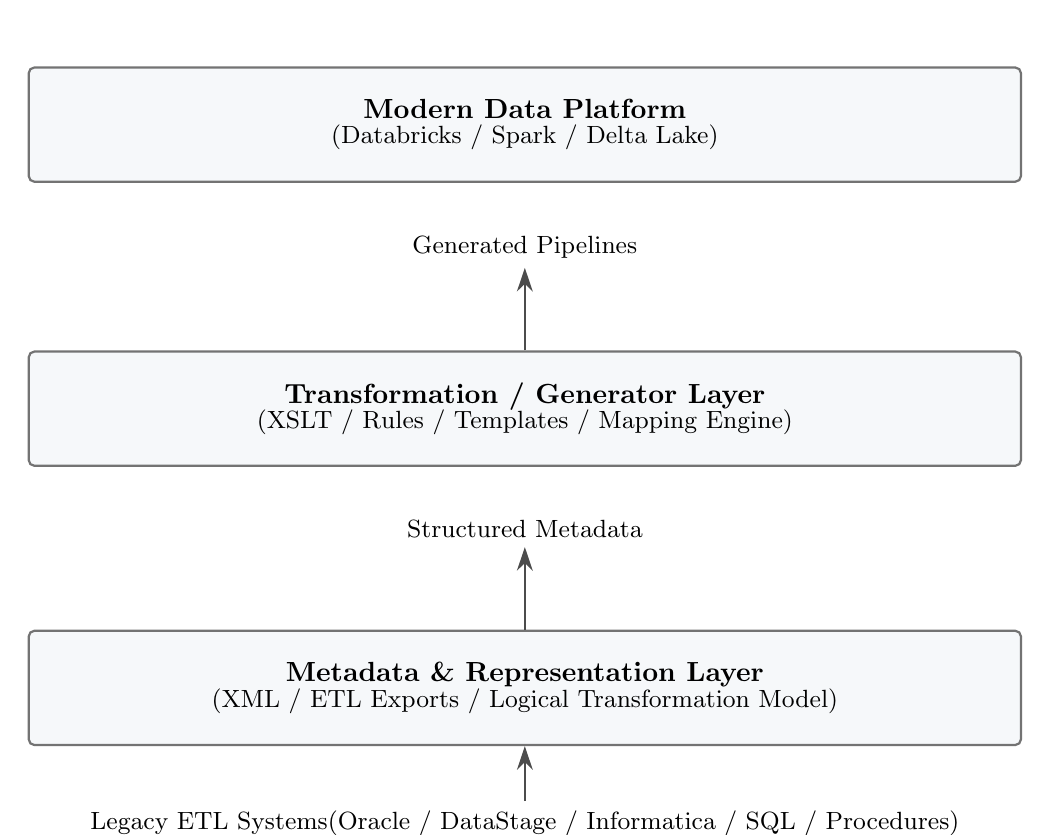
\begin{tikzpicture}[node distance=1.55cm]
    \node (modern) [hfbox] {\textbf{Modern Data Platform}\\[-1mm]\small (Databricks / Spark / Delta Lake)};
    \node (txt1) [below=0.55cm of modern, hfsmall] {Generated Pipelines};
    \node (generator) [hfbox, below=1.05cm of txt1] {\textbf{Transformation / Generator Layer}\\[-1mm]\small (XSLT / Rules / Templates / Mapping Engine)};
    \node (txt2) [below=0.55cm of generator, hfsmall] {Structured Metadata};
    \node (meta) [hfbox, below=1.05cm of txt2] {\textbf{Metadata \& Representation Layer}\\[-1mm]\small (XML / ETL Exports / Logical Transformation Model)};
    \node (legacytxt) [below=0.7cm of meta, hfsmall] {Legacy ETL Systems\\[-1mm]\small (Oracle / DataStage / Informatica / SQL / Procedures)};

    \draw[hfarrow] (generator.north) -- (txt1.south);
    \draw[hfarrow] (meta.north) -- (txt2.south);
    \draw[hfarrow] (legacytxt.north) -- (meta.south);
  \end{tikzpicture}
  \caption{Conceptual architecture of the generator-based lift-and-shift approach.}
  \label{fig:conceptual-architecture}
\end{figure}


\subsection{Legacy Extraction Layer}

The process starts with existing ETL systems.

Typical sources include:
\begin{itemize}
  \item DataStage job definitions (XML exports),
  \item Oracle-based ETL logic (PL/SQL, SQL scripts),
  \item Informatica workflows and mappings.
\end{itemize}

These artifacts are not executed directly. Instead, they are extracted and interpreted as structured representations of logic.

The goal is not to replicate execution, but to capture intent.

\subsection{Metadata and Representation Layer}

Extracted artifacts are normalized into a structured, machine-readable form.

This representation includes:
\begin{itemize}
  \item source-to-target mappings,
  \item transformation expressions,
  \item join conditions and filters,
  \item key definitions (BK/SK),
  \item temporal validity rules,
  \item process-specific parameters.
\end{itemize}

This layer acts as a canonical model of transformation logic, independent of any specific execution engine.

It provides a consistent foundation for further processing.

\subsection{Transformation / Generator Layer}

The generator layer is the core of the architecture.

Here, structured metadata is processed using deterministic transformation rules.

Typical mechanisms include:
\begin{itemize}
  \item XSLT-based transformations,
  \item rule-driven mapping logic,
  \item template-based code generation.
\end{itemize}

The generator produces:
\begin{itemize}
  \item Spark SQL statements,
  \item PySpark transformations,
  \item standardized pipeline structures.
\end{itemize}

Each generated artifact follows predefined architectural patterns, ensuring consistency across all pipelines.

\subsection{Execution Layer (Databricks / Spark)}

Generated pipelines are executed on a modern data platform, such as Databricks.

Key characteristics:
\begin{itemize}
  \item separation between generated code and runtime execution,
  \item integration with Delta Lake (ACID, versioning),
  \item scalable processing using Spark,
  \item orchestration via jobs or workflows.
\end{itemize}

Because pipelines are generated rather than manually implemented, the execution layer remains clean, consistent, and aligned with platform best practices.

\subsection{Cross-Cutting Concerns}

The architecture allows standardized handling of recurring concerns:
\begin{itemize}
  \item surrogate key generation (e.g.\ hash-based SK),
  \item temporal validity (e.g.\ SCD Type 2 patterns),
  \item auditing and lineage,
  \item parameterization and environment handling,
  \item naming conventions and structure.
\end{itemize}

These aspects are implemented once in the generator and applied consistently across all pipelines.

\subsection{Summary}

The architecture separates extraction, representation, transformation, and execution into distinct layers.

This enables:
\begin{itemize}
  \item controlled transformation of legacy logic,
  \item consistent pipeline generation,
  \item scalable execution on modern platforms.
\end{itemize}

Most importantly, it provides a foundation for evolving towards structured, data product-oriented architectures.

\section{Example Transformation: A Real-World Enterprise Modernization Pattern}

To make the approach concrete, this section outlines a transformation pattern derived from a real enterprise modernization initiative in a regulated environment.

The example is intentionally abstracted. It does not describe a specific company, schema, or process, but reflects an implementation pattern used to migrate legacy ETL logic from a traditional on-premise stack into a Databricks-based target architecture.

The purpose of the example is not to showcase a single pipeline, but to illustrate how a generator-based lift-and-shift approach can systematically transform legacy process definitions into modern, executable data pipelines.

\subsection{Initial Situation}

The starting point was a legacy ETL landscape with the following characteristics:
\begin{itemize}
  \item business-critical data flows implemented in a traditional ETL tool,
  \item source and target mappings defined in exported XML process definitions,
  \item transformation logic distributed across ETL stages, SQL expressions, and database-specific constructs,
  \item strong dependence on existing naming, sequencing, and validity-handling conventions,
  \item extensive reuse of established business logic that could not simply be discarded and rebuilt from scratch.
\end{itemize}

From a migration perspective, the challenge was clear: the logic was already proven in production, but its implementation was tied to a legacy execution model.

A manual rebuild in the target platform would have required significant effort, introduced interpretation risk, and reduced consistency across migrated processes.

\subsection{Generator Input}

Instead of rewriting the pipelines manually, the exported process definitions were used as structured input to a generator framework.

The generator consumed metadata such as:
\begin{itemize}
  \item source and target entities,
  \item business keys and technical keys,
  \item join conditions and filter expressions,
  \item column mappings and derived expressions,
  \item temporal validity rules,
  \item step structure of the original ETL process.
\end{itemize}

This input was interpreted not as executable code, but as a formal description of transformation intent.

That distinction is essential: the objective was not to preserve the legacy runtime, but to preserve the logic while relocating execution to a modern platform.

\subsection{Transformation Principle}

The transformation followed a rule-based pattern.

Legacy constructs were mapped to standardized target patterns, for example:
\begin{itemize}
  \item legacy null-handling functions mapped to ANSI-compliant SQL expressions,
  \item sequence-based surrogate key logic mapped to deterministic hash-based key generation,
  \item temporal validity handling mapped to standardized validity windows in Spark / Delta,
  \item step-oriented ETL flows mapped to generated Spark SQL views and controlled merge steps,
  \item tool-specific implementation details removed or replaced by target-platform conventions.
\end{itemize}

This allowed the generator to produce pipelines that were structurally modern, while remaining logically aligned with the original process definitions.

\subsection{Target Execution Model}

The generated output was aligned with a Databricks-based execution architecture.

In simplified terms, the generated pipelines followed this pattern:
\begin{enumerate}
  \item ingest and expose intermediate transformation steps as standardized temporary views,
  \item apply transformation logic using generated Spark SQL,
  \item handle business keys, surrogate keys, and temporal validity through reusable patterns,
  \item merge the final result into Delta target tables using controlled write semantics.
\end{enumerate}

This approach ensured that execution remained platform-native, while pipeline creation remained metadata-driven.

\subsection{Simplified Example}

The following simplified example illustrates the principle.

A legacy process defines:
\begin{itemize}
  \item a source entity representing business objects,
  \item derived fields based on source expressions,
  \item a business key composed of multiple attributes,
  \item a technical target table with validity handling,
  \item a final load into the curated target structure.
\end{itemize}

Conceptually, the metadata may be represented as follows:

\begin{lstlisting}[style=hfcode,caption={Simplified metadata representation.}]
process:
  source: BUSINESS_OBJECT_RAW
  target: BUSINESS_OBJECT_CURATED

  business_key:
    - BUSINESS_ID
    - LOCATION_ID
    - PROCESS_ID

  transformations:
    OBJECT_NAME: SOURCE.NAME
    OBJECT_TYPE: SOURCE.TYPE
    VALID_FROM: SOURCE.LOAD_TS
    VALID_TO: HIGH_VALUE_TIMESTAMP

  filters:
    - SOURCE.STATUS = 'ACTIVE'

  temporality:
    type: scd2
    valid_from: VALID_FROM
    valid_to: VALID_TO
\end{lstlisting}

From this metadata, the generator derives standardized Spark-based transformation steps.

A simplified conceptual output could look as follows:

\begin{lstlisting}[style=hfcode,language=SQL,caption={Conceptual generated Spark SQL output.}]
CREATE OR REPLACE TEMP VIEW V_STEP_01_BUSINESS_OBJECT AS
SELECT
    abs(xxhash64(BUSINESS_ID, LOCATION_ID, PROCESS_ID)) AS OBJECT_SK,
    SOURCE.NAME AS OBJECT_NAME,
    SOURCE.TYPE AS OBJECT_TYPE,
    SOURCE.LOAD_TS AS VALID_FROM,
    to_timestamp('9999-12-31 23:59:59') AS VALID_TO
FROM BUSINESS_OBJECT_RAW SOURCE
WHERE SOURCE.STATUS = 'ACTIVE';
\end{lstlisting}

Followed by a controlled merge into the curated Delta target:

\begin{lstlisting}[style=hfcode,language=SQL,caption={Conceptual generated Delta merge output.}]
MERGE INTO BUSINESS_OBJECT_CURATED t
USING V_STEP_01_BUSINESS_OBJECT s
ON t.OBJECT_SK = s.OBJECT_SK
WHEN MATCHED THEN UPDATE SET ...
WHEN NOT MATCHED THEN INSERT ...;
\end{lstlisting}

This example is simplified, but it captures the essential point: the target pipeline is not handwritten. It is generated from a structured representation of the legacy process.

\subsection{What This Demonstrates}

This real-world pattern demonstrates several important aspects of the approach:
\begin{itemize}
  \item existing ETL definitions can serve as generator input,
  \item validated business logic can be preserved without manual line-by-line migration,
  \item legacy implementation details can be replaced by standardized target patterns,
  \item execution can be modernized without losing structural control over the transformation.
\end{itemize}

Most importantly, the migration becomes repeatable.

Instead of treating each process as an isolated implementation effort, the organization gains a framework for systematic modernization across many pipelines.

\subsection{Summary}

A generator-based lift-and-shift approach is particularly effective in enterprise environments where legacy ETL logic is mature, business-critical, and deeply embedded in existing systems.

By using real process definitions as structured input and applying deterministic transformation rules, organizations can move to modern platforms in a way that is both pragmatic and architecturally controlled.

This turns migration from a manual rewrite exercise into a scalable transformation discipline.

\section{Benefits and Trade-offs}

A generator-based lift-and-shift approach provides a structured and scalable path for modernizing legacy data platforms. However, like any architectural approach, it introduces both advantages and trade-offs.

Understanding these aspects is essential for evaluating where and how this approach can be applied effectively.

\subsection{Benefits}

\subsubsection{Consistency and Standardization}

By generating pipelines from structured metadata and deterministic rules, all transformations follow the same architectural patterns.

This leads to:
\begin{itemize}
  \item consistent naming conventions and pipeline structures,
  \item uniform handling of keys, temporality, and data flows,
  \item reduced variability between implementations.
\end{itemize}

Consistency is particularly important in large-scale environments, where manual implementations tend to diverge over time.

\subsubsection{Repeatability and Scalability}

Once the transformation rules are defined, they can be applied to many processes without additional implementation effort.

This enables:
\begin{itemize}
  \item systematic migration of large numbers of ETL processes,
  \item predictable outcomes across different domains,
  \item reduced dependency on individual developers.
\end{itemize}

Migration becomes a repeatable process rather than a series of isolated projects.

\subsubsection{Preservation of Validated Business Logic}

Legacy ETL systems often contain years of accumulated domain knowledge.

A generator-based approach allows this logic to be preserved while changing its execution model.

This reduces:
\begin{itemize}
  \item interpretation risk during migration,
  \item loss of implicit business rules,
  \item need for full functional revalidation.
\end{itemize}

This is particularly valuable in regulated environments, where correctness is critical.

\subsubsection{Separation of Logic and Execution}

By externalizing transformation logic into metadata and rules, the approach clearly separates:
\begin{itemize}
  \item business logic,
  \item technical implementation.
\end{itemize}

This improves:
\begin{itemize}
  \item maintainability,
  \item transparency,
  \item adaptability to new platforms.
\end{itemize}

Changes to execution technology no longer require rewriting transformation logic.

\subsubsection{Faster Time-to-Migration}

Compared to manual reimplementation, generator-based approaches can significantly reduce migration time.

Effort shifts from writing pipelines to defining and refining transformation rules.

Once the framework is established, additional processes can be migrated with relatively low incremental effort.

\subsubsection{Foundation for Further Evolution}

Although initially focused on migration, the structured representation of logic creates a foundation for:
\begin{itemize}
  \item data product-oriented architectures,
  \item improved lineage and traceability,
  \item automated validation and testing,
  \item integration with governance frameworks.
\end{itemize}

The approach supports not only migration, but also long-term evolution.

\subsection{Trade-offs and Limitations}

\subsubsection{Initial Investment in the Generator Framework}

The approach requires upfront effort to design and implement:
\begin{itemize}
  \item metadata models,
  \item transformation rules,
  \item generation templates.
\end{itemize}

This investment must be justified by the scale of migration and expected reuse.

For small environments, a manual approach may be more efficient.

\subsubsection{Coverage of Legacy Constructs}

Legacy ETL systems often contain edge cases, custom logic, or tool-specific features.

Not all constructs can be directly mapped to standardized patterns.

This may require:
\begin{itemize}
  \item extending transformation rules,
  \item introducing fallback mechanisms,
  \item handling exceptions outside the generator.
\end{itemize}

Complete coverage is rarely achieved in a single iteration.

\subsubsection{Abstraction Overhead}

Introducing a metadata and generator layer adds an additional level of abstraction.

This can:
\begin{itemize}
  \item increase initial complexity,
  \item require new skills and understanding,
  \item make debugging less direct compared to handwritten code.
\end{itemize}

Proper tooling and documentation are essential to manage this complexity.

\subsubsection{Risk of Over-Standardization}

While standardization is a strength, it can also become a limitation.

Strict patterns may:
\begin{itemize}
  \item reduce flexibility for specific use cases,
  \item constrain optimizations for particular workloads,
  \item enforce structures that are not always optimal.
\end{itemize}

A balance must be maintained between consistency and adaptability.

\subsubsection{Not a Replacement for Architectural Decisions}

A generator-based approach does not eliminate the need for architectural design.

Decisions such as:
\begin{itemize}
  \item data modeling strategy,
  \item domain boundaries,
  \item data product ownership,
  \item platform governance.
\end{itemize}

remain essential and must be addressed separately.

The generator supports implementation, but does not replace architecture.

\subsection{Summary}

A generator-based lift-and-shift approach offers a pragmatic and scalable method for modernizing legacy ETL systems, particularly in large and complex environments.

Its strengths lie in consistency, repeatability, and the preservation of existing logic.

However, it requires upfront investment, careful design, and an understanding of its limitations.

When applied appropriately, it provides not only a migration path, but a foundation for more structured and maintainable data platforms.

\section{Outlook: From Structured Transformation to Data Products}

The generator-based lift-and-shift approach described in this paper is not an end state. It is a transitional architecture that addresses one of the most critical challenges in modern data platform initiatives: how to move from legacy systems to scalable, maintainable environments without losing control over existing logic.

By introducing structure, repeatability, and separation of concerns, this approach establishes a foundation that goes beyond migration.

It creates the conditions for a more fundamental shift: from pipeline-centric systems to data product-oriented architectures.

\subsection{From Pipelines to Data Products}

In traditional environments, data pipelines are often treated as technical implementations.

They are built to move and transform data, but they rarely have:
\begin{itemize}
  \item clear ownership,
  \item defined interfaces,
  \item explicit lifecycle management,
  \item consistent quality guarantees.
\end{itemize}

As a result, data consumers depend on implicit knowledge and fragile dependencies.

By contrast, modern data architectures—often described in the context of Data Mesh—emphasize \emph{data products}:
\begin{itemize}
  \item domain-owned,
  \item well-defined and discoverable,
  \item governed and versioned,
  \item designed for reuse.
\end{itemize}

A generator-based approach supports this transition by making transformation logic explicit and structured.

Instead of pipelines being opaque implementations, they become reproducible artifacts derived from well-defined models.

\subsection{Enabling Structured Ownership and Governance}

When transformation logic is externalized and standardized, it becomes possible to introduce clearer ownership models.

This includes:
\begin{itemize}
  \item assigning responsibility for specific data domains,
  \item defining consistent interfaces between data producers and consumers,
  \item enforcing common standards across teams,
  \item improving traceability and lineage.
\end{itemize}

The generator layer acts as a control point where such standards can be defined and consistently applied.

This is a key enabler for scaling data platforms across organizational boundaries.

\subsection{Towards Platform-Level Capabilities}

The concepts described in this paper can be extended beyond individual transformations.

A natural evolution is the development of a platform that:
\begin{itemize}
  \item manages metadata as a central asset,
  \item provides interfaces for defining and evolving transformation logic,
  \item automates generation, validation, and deployment of pipelines,
  \item integrates with execution environments such as Databricks.
\end{itemize}

In such a setup, the generator is no longer just a migration tool, but part of a broader system for managing data processing as a structured discipline.

\subsection{HeptaFlow: A Conceptual Direction}

The ideas outlined in this paper form the foundation for a broader vision, referred to here as \emph{HeptaFlow}.

HeptaFlow represents a conceptual evolution towards:
\begin{itemize}
  \item metadata-driven data platform design,
  \item generator-based pipeline creation,
  \item integrated validation and consistency checks,
  \item structured support for data product architectures.
\end{itemize}

At its core, the goal is to treat transformation logic not as scattered implementation detail, but as a governed, reusable, and evolvable asset.

While the current approach focuses on controlled transformation and migration, the long-term direction is to enable a more comprehensive platform that supports the full lifecycle of data products.

\subsection{Final Perspective}

Modernizing data platforms is not only a technical challenge, but an architectural one.

Organizations that focus solely on migrating pipelines risk reproducing legacy complexity in a new environment.

By introducing structured transformation, deterministic generation, and clear separation of concerns, it becomes possible to move beyond migration towards a more sustainable model.

A generator-based lift-and-shift approach provides a pragmatic starting point.

From there, the path leads toward data platforms that are not only modern in technology, but also structured, transparent, and aligned with how data is actually used across the organization.

\section*{Conclusion}
\addcontentsline{toc}{section}{Conclusion}

Legacy ETL modernization is often framed as a tooling problem. In practice, it is a structural challenge.

A generator-based lift-and-shift approach offers a pragmatic path forward by preserving proven business logic while transforming the way it is represented, governed, and executed. This makes modernization more consistent, more scalable, and better aligned with long-term architectural goals.

For organizations facing large-scale migration from legacy ETL systems to platforms such as Databricks, the key question is not simply how to move pipelines, but how to establish a controlled transformation model that prevents legacy complexity from being recreated in a new environment.

That is where generator-based modernization becomes more than a migration technique. It becomes the starting point for a more disciplined data platform architecture.

\end{document}
